%Do not alter this block of commands.  If you're proficient at LaTeX, you may include additional packages, create macros, etc. immediately below this block of commands, but make sure to NOT alter the header, margin, and comment settings here. 
\documentclass[12pt]{article}
 \usepackage[margin=1in, bottom=4.5cm]{geometry}
\usepackage{amsmath,amsthm,amssymb,amsfonts, enumitem, fancyhdr, color, comment, graphicx, environ, scrextend}
\usepackage[table,dvipsnames]{xcolor}
\usepackage{tikz}  
\usepackage{tikz-3dplot} 
\usepackage{amssymb}
\usepackage{xifthen}
\pagestyle{fancy}
\setlength{\headheight}{65pt}
\newenvironment{problem}[2][Problem]{\begin{trivlist}
\item[\hskip \labelsep {\bfseries #1}\hskip \labelsep {\bfseries #2.}]}{\end{trivlist}}
\newenvironment{sol}
    {\emph{Proof.}
    }
    {
    \qed
    }
\specialcomment{com}{ \color{blue} \textbf{Comment:} }{\color{black}} %for instructor comments while grading
\NewEnviron{probscore}{\marginpar{ \color{blue} \tiny Problem Score: \BODY \color{black} }}
%%%%%%%%%%%%%%%%%%%%%%%%%%%%%%%%%%%%%%%%%%%%%%%%%%%%%%%%%%%%%%%%%%%%%%%%%%%%%%%%%

\newcommand\restr[2]{{% we make the whole thing an ordinary symbol
  \left.\kern-\nulldelimiterspace % automatically resize the bar with \right
  #1 % the function
  \vphantom{\big|} % pretend it's a little taller at normal size
  \right|_{#2} % this is the delimiter
  }}





%%%%%%%%%%%%%%%%%%%%%%%%%%%%%%%%%%%%%%%%%%%%%
%Fill in the appropriate information below
\lhead{Trey Manuszak}  %replace with your name
\rhead{MAT 473: Intermediate Real Analysis II \\ Homework 7: 25, 26, 27, 28} %replace XYZ with the homework course number, semester (e.g. ``Spring 2019"), and assignment number.
%%%%%%%%%%%%%%%%%%%%%%%%%%%%%%%%%%%%%%%%%%%%%

\usepackage{blindtext}
\title{MAT 473: Intermediate Real Analysis II}
\date{March 19, 2020}
\author{Trey Manuszak\\ Arizona State University}



%%%%%%%%%%%%%%%%%%%%%%%%%%%%%%%%%%%%%%
%Do not alter this block.
\begin{document}
%%%%%%%%%%%%%%%%%%%%%%%%%%%%%%%%%%%%%%




\maketitle
\newpage



%Solutions to problems go below.  Please follow the guidelines from https://www.overleaf.com/read/sfbcjxcgsnsk/


%Copy the following block of text for each problem in the assignment.
\begin{problem}{25}
Let $p,q \geq 1$ with $\frac{1}{p} + \frac{1}{q} = 1$. \begin{itemize}
    \item[(a)] Use the method of Lagrange multipliers to find the minimum of $\frac{1}{p}x^p + \frac{1}{q}y^q$ subject to the constraints $xy = 1$ and $x > 0$.
    
    \begin{sol}
    Taking each partial derivative, we must find a Lagrange multiplier $\lambda$ such that \begin{align}
        x^{p-1} - \lambda y &= 0 \\ y^{q-1} - \lambda x &= 0.
    \end{align} Note, $x = \frac{1}{y}$ and $y = \frac{1}{x}$. So, adding $\lambda y$ and multiplying by $x$, or $\frac{1}{y}$, to equation (1), we get $x^p = \lambda$. Similarly with equation (2), we get $y^q = \lambda$. Since $xy = 1$, then $x = y = 1$. Therefore, the minimum of $\frac{1}{p}x^p + \frac{1}{q}y^q$ subject to the constraints $xy = 1$ and $x > 0$ with $p,q \geq 1$ and $\frac{1}{p} + \frac{1}{q} = 1$ is $\frac{1}{p} + \frac{1}{q} = 1$.
    \end{sol}
    
    \item[(b)] Prove that $\frac{1}{p}x^p + \frac{1}{q}y^q \geq xy$ for all $x,y \geq 0$.
    
    \begin{sol}
    Clearly, it is true if either $x$ or $y$ are zero, so suppose $x$ and $y$ are greater than zero. Note, if $(x,y)$ satisfy the inequality, then all numbers of the form $xr^{\frac{1}{p}}$ and $yr^{\frac{1}{q}}$ are true for any $r \in \mathbb{R}^+$. Thus, we may restrict ourselves such that $xy = 1$, which implies we want to show that for all $x,y \in \mathbb{R}^+$ with $xy=1$, we get $$\frac{1}{p}x^p + \frac{1}{q}y^q \geq 1.$$ 
    
    \hspace{1em} So, we must see if the minimum of $\frac{1}{p}x^p + \frac{1}{q}y^q$ subject to the constraints exists. This is exactly part (a). Thus, $\frac{1}{p}x^p + \frac{1}{q}y^q \geq xy$ for all $x,y \geq 0$.
    \end{sol}
    
    \item[(c)] Prove H\"older's inequality: if $u_i, v_i \geq 0$ for $i = 1, \dots, n$, then $$\sum_{i = 1}^nu_iv_i \leq \left( \sum_{i = 1}^n u_i^p \right)^{\frac{1}{p}} \left( \sum_{i = 1}^n v_i^q \right)^{\frac{1}{q}}.$$ (Hints: for $u = (u_1, \dots, u_n)$ let $\lVert u \rVert_p = \left( \sum_{i = 1}^n u_i^p \right)^{\frac{1}{p}}$ . If $\lVert u \rVert_p, \lVert v \rVert_q \neq 0$, let $x = \frac{u_i}{\lVert u \rVert_p}$ and $\frac{v_i}{\lVert v \rVert_q}$ in part (b).)
    
    \begin{sol}
    Let $$u = \frac{u_i}{\left( \sum_{i = 1}^n u_i^p \right)^{\frac{1}{p}}} \hspace{2em} \text{and} \hspace{2em} v = \frac{v_i}{\left( \sum_{i = 1}^n v_i^q \right)^{\frac{1}{q}}},$$ such that $u_1,u_2,\dots,u_n,v_1,v_2,\dots,v_n \in \mathbb{R}^+$ and each component of $(u,v)$ nonzero. Then, by Young's inequality, which is part (b), we get
    \begin{align*}
        \sum_{i = 1}^n \left| u_iv_i \right| &\leq \sum_{i = 1}^n \left( \frac{u_i^p}{p} + \frac{v_i^q}{q} \right).
    \end{align*}
    Using the fact that $\frac{1}{p} + \frac{1}{q} = 1$, we get $\sum_{i = 1}^n \left| u_iv_i \right| \leq 1$. One can also show that $\sum_{i = 1}^nu_i^p = 1$ and $\sum_{i = 1}^nv_i^p = 1$. Therefore, we get H\"older's inequality $$\sum_{i = 1}^nu_iv_i \leq \left( \sum_{i = 1}^n u_i^p \right)^{\frac{1}{p}} \left( \sum_{i = 1}^n v_i^q \right)^{\frac{1}{q}}.$$
    \end{sol}
\end{itemize}
\end{problem}


\begin{problem}{26}
Let $f : \mathbb{R}^2 \to \mathbb{R}^2$ be given by $f(x) = (e^{x_1}\cos x_2,e^{x_1}\sin x_2).$ \begin{itemize}
    \item[(a)] Find (with proof) the range of $f$.
    
    \begin{sol}
    Consider the following sets: $Z_1 = \mathbb{R}_* \times \mathbb{R}$ and $Z_2 = \mathbb{R} \times \mathbb{R}_*$. For $a \in Z_1$ or $a \in Z_2$, let $g_1 : Z_1 \to \mathbb{R}_*^2$ be defined by $g_1(a) = f(b_1,b_2)$ and let $g_2 : Z_2 \to \mathbb{R}_*^2$ be defined by $g_2(a) = f(b_1,b_2)$, respectively such that $b_1 = \ln \left( \sqrt{a_1^2 + a_2^2} \right)$ and $$b_2 = \begin{cases} 
      \tan^{-1} \left( \frac{a_2}{a_1} \right), & \text{if } a_1 \neq 0 \\
      \cot^{-1}\left( \frac{a_1}{a_2} \right), & \text{if } a_2 \neq 0.
   \end{cases}$$
   \hspace{1em} Without loss of generality, since it can be shown similarly in both cases, let $a \in Z_1$. Then, \begin{align*}
       g_1(a) &= f(b_1,b_2) \\ 
       &= \left( e^{\ln \left( \sqrt{a_1^2 + a_2^2} \right)}\cos \left( \tan^{-1} \left( \frac{a_2}{a_1} \right) \right), e^{\ln \left( \sqrt{a_1^2 + a_2^2} \right)}\sin \left( \tan^{-1} \left( \frac{a_2}{a_1} \right) \right) \right)\\ 
       &= \left( \sqrt{a_1^2 + a_2^2} \left( \frac{a_1}{\sqrt{a_1^2 + a_2^2}} \right) , \sqrt{a_1^2 + a_2^2} \left( \frac{a_2}{\sqrt{a_1^2 + a_2^2}} \right) \right) \\ 
       &= (a_1,a_2).
   \end{align*}
   Thus, $f$ is surjective if we consider the codomain to be $\mathbb{R}_*^2$. 
   Also, clearly, we cannot have $0 \in \text{ran}f$ since $e^{x_1} > 0$ for all $x_1 \in \mathbb{R}$ and if $\sin x_2 = 0$, then $\cos x_2 \neq 0$. Therefore, exhausting all possibilities, we have $\text{ran}f = \mathbb{R}_*^2$.
    \end{sol}
    
    \item[(b)] Prove that $f'(x)$ is non-singular for every $x \in \mathbb{R}^2$, but that $f$ is not one-to-one.
    
    \begin{sol}
    Let $f : \mathbb{R}^2 \to \mathbb{R}^2$ be defined by $f(x) = (e^{x_1}\cos x_2,e^{x_1} \sin x_2)$. Then, $$f'(x) = \begin{pmatrix}
        e^{x_1} \cos x_2 & -e^{x_1} \sin x_2 \\ 
        e^{x_1} \sin x_2 & e^{x_1} \cos x_2
    \end{pmatrix}.$$ Now, \begin{align*}
        \left| \begin{pmatrix}
        e^{x_1} \cos x_2 & -e^{x_1} \sin x_2 \\ 
        e^{x_1} \sin x_2 & e^{x_1} \cos x_2
    \end{pmatrix} \right| &= e^{2x_1} \cos^2 x_2 + e^{2x_1} \sin^2 x_2 \\ &= e^{2x_1}.
    \end{align*}
    Since $e^{2x_1} > 0$ for all $x_1 \in \mathbb{R}$, then $f'(x)$ is always non-singular. Also, since neither $\cos$ nor $\sin$ are injective on $\mathbb{R}$, then $f$ is not injective.
    \end{sol}
    
    \item[(c)] Let $U = \{x \in \mathbb{R}^2 : \left| x_2 \right| < \pi \}$. Prove that $\restr{f}{U}$ is one-to-one, and find $f(U)$. Also prove that for any open set $V$ properly containing $U$, $\restr{f}{V}$ is not one-to-one.
    
    \begin{sol}
    Let $U = \{x \in \mathbb{R}^2 : \left| x_2 \right| < \pi \} = \{x \in \mathbb{R}^2 : x_2 \in (-\pi,\pi)\}$. Let $x,y \in U$ such that $f(x) = f(y)$. Then, 
    \begin{align*}
       e^{x_1}\cos x_2 &= e^{y_1}\cos y_2 &\hspace{3em} e^{x_1}\sin x_2 &= e^{y_1}\sin y_2 \\ e^{2x_1}\cos^2 x_2 &= e^{2y_1}\cos^2 y_2 &\hspace{3em} e^{2x_1}\sin^2 x_2 &= e^{2y_1}\sin^2 y_2. \tag*{(By squaring both sides)}
    \end{align*} 
    By adding the two equations together, we get $$e^{2x_1}\cos^2 x_2 + e^{2x_1}\sin^2 x_2 = e^{2y_1}\cos^2 y_2 + e^{2y_1}\sin^2 y_2,$$ which simplifies to $e^{2x_1} = e^{2y_1}$. These are injective functions, which implies $x_1 = y_1$. By substitution, we get $e^{x_1}\cos x_2 = e^{x_1}\cos y_2$ and $e^{x_1}\sin x_2 = e^{x_1}\sin y_2$. By division, we have $\cos x_2 = \cos y_2$ and $\sin x_2 = \sin y_2$. This is broken down in the following cases:
    
    \begin{itemize}
        \item[\underline{Case 1:}] $x_2 \in (-\pi,0)$:
        \begin{itemize}
            \item[\underline{Case 1a:}] Let $y_2 \in (-\pi,0)$. Note, $\cos$ is injective on this interval, so $\cos x_2 = \cos y_2$ implies $x_2 = y_2$.
            
            \item[\underline{Case 1b:}] Let $y_2 \in [0,\pi)$. Since $\sin x_2 < 0$ and $\sin y_2 \geq 0$, then $\sin x_2 \neq \sin y_2$, which is impossible.
        \end{itemize}
        
        \item[\underline{Case 2:}] $x_2 \in [0,\pi)$:
        \begin{itemize}
            \item[\underline{Case 1a:}] Let $y_2 \in (-\pi,0)$. Since $\sin x_2 \geq 0$ and $\sin y_2 < 0$, then $\sin x_2 \neq \sin y_2$, which is impossible.
            
            \item[\underline{Case 1b:}] Let $y_2 \in [0,\pi)$. Note, $\cos$ is injective on this interval, which implies $\cos x_2 = \cos y_2$, which implies $x_2 = y_2$.
        \end{itemize}
    \end{itemize}
    
    So, in all possible cases, we have $x_2 = y_2$. Therefore, $x = y$. Thus, $\restr{f}{U}$ is injective.
    
    \hspace{1em}Now, let $a \in \mathbb{R}_*^2$. Also, let $b_1 = \ln \left( \sqrt{a_1^2 + a_2^2} \right)$ and $$b_2 = \begin{cases} 
      \tan^{-1} \left( \frac{a_2}{a_1} \right), & \text{if } a_1 \neq 0 \\
      \cot^{-1}\left( \frac{a_1}{a_2} \right), & \text{if } a_2 \neq 0.
   \end{cases}$$ Note, $b \in U$ since the range of $\tan^{-1}$ and $\cot^{-1}$ is $(\frac{-\pi}{2},\frac{\pi}{2})$. From (a), we know that $f(b) = a$. So, $\text{ran}\left(\restr{f}{U}\right) \supseteq \mathbb{R}_*^2$.However, the cardinality of the range cannot be larger when the domain is restricted. Thus, $$\text{ran}\left(\restr{f}{U}\right) = \mathbb{R}_*^2.$$
   
   \hspace{1em} Now, suppose $V \subseteq \mathbb{R}^2$ open such that $U \subset V$. Then, there exists $q \in V \setminus U$. Let $$E = \begin{cases} 
      \{q_2 + 2\pi k : k \in \mathbb{Z},q_2 \geq q_2 + 2\pi k > -\pi\}, & \text{if } q_2 \geq \pi \\
      \{q_2 + 2\pi k : k \in \mathbb{Z},\pi > q_2 + 2 \pi k \geq q_2\}, & \text{if } q_2 \leq -\pi.
   \end{cases}$$
    \hspace{1em} Suppose, without loss of generality, that $q_2 \geq \pi$. Now, $E$ is finite and $E \neq \emptyset$, since $q_2 \in E$. Let $m = \min E$. Then, if $m \not \in U$, then $m = \pi$, else $m - 2\pi \in E$, which is a contradiction. If $m \in U$, let $u_2 = m$ with $u \in U$. Else, there exists $r > 0$ such that $B_r(q_1,q_2) \subseteq V$ since $V$ is open.
    
    \hspace{1em} Let $p = \min\{q_2 + \frac{r}{2}, q_2 + \frac{3\pi}{2}\}$. So, $(q_1,p) \in V$. Also, there exists $k \in \mathbb{Z}$ such that $q_2 + 2 \pi k = m$ since $m \in E$, which implies $$\pi = m = q_2 + 2 \pi k < p + 2 \pi k \leq q_2 + \frac{3\pi}{2} + 2\pi k = m + \frac{3 \pi}{2} = \frac{5 \pi}{2}.$$ By subtracting $2 \pi$, we get $-\pi < p + 2 \pi (k-1) \leq \frac{3 \pi}{2}$, which implies $(q_1,p+2\pi (k-1)) \in U$. If this is the case, let $u_2 = p + 2 \pi (k-1)$. Either way, we have $(q_1,u_2) \in V$ and $(q_1,u_2 + 2 \pi \alpha) \in U \subset V$ for some $\alpha \in \mathbb{Z}$. So, \begin{align*}
        f(q_1,u_2) &= (e^{q_1}\cos u_2, e^{q_1} \sin u_2) \\ &= (e^{q_1} \cos (u_2 + 2 \pi \alpha),e^{q_1} \sin (u_2 + 2 \pi \alpha)) \\ &= f(q_1,u_2 + 2\pi \alpha).
    \end{align*}
    Therefore, $\restr{f}{V}$ is not injective.
    \end{sol}
\end{itemize}
\end{problem}


\begin{problem}{27}
Let $f : \mathbb{R}^2 \to \mathbb{R}$ be continuously differentiable. In each part, the portion of the level set $\{x \in \mathbb{R}^2 : f(x) = 0\}$ is sketched near a point on the level set. What can you say about the derivatives $f'(A)$ and $f'(B)$? Justify your answers precisely.

\begin{center}
    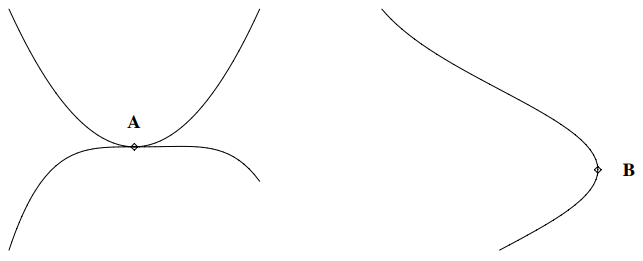
\includegraphics[scale=1]{473figure.PNG}
    \end{center}
    
    \begin{sol}
    Note, the important thing to consider with the two diagrams is whether, for $x = (x_1,x_2) \in \mathbb{R}^2$, $x_1$ can be represented as a function of $x_2$ or if $x_2$ can be represented as a function of $x_1$. Considering the diagram with point $A$, there clearly does not exist a function that can approximate one variable with the other. Thus, $D_1f(A) = D_2f(A) = 0$. As for the diagram with point $B$, $x_1$ can be represented as a function of $x_2$, but $x_2$ can not be represented as a function of $x_1$. Therefore, $D_2f(B) = 0$.
    \end{sol}
\end{problem}


\begin{problem}{28}
Let $f : U \subseteq \mathbb{R}^3 \to \mathbb{R}^2$ be continuously differentiable, let $a \in U$, and suppose that $\frac{\partial f}{\partial (x_2,x_3)}(a)$ is non-singular (as a $2 \times 2$ matrix). Prove that there are open subsets $V$ and $W$ of $\mathbb{R}^3$ with $a \in W$, and a $C^1$-diffeomorphism $h : V \to W$, such that $f \circ h(x) = (x_2, x_3)$ for all $x \in V$. (Hint: let $F(x) = (x_1,f(x))$ and use the inverse function theorem.)
\end{problem}

\begin{sol}
Let $f : U \subseteq \mathbb{R}^3 \to \mathbb{R}^2$ be continuously differentiable, let $a \in U$, and suppose that $\frac{\partial f}{\partial (x_2,x_3)}(a) \in M_2$ is non-singular. Define $F : \mathbb{R}^3 \to \mathbb{R}^3$ by $F(x) = (x_1,f(x))$. Since $\frac{\delta f}{\delta (a_2,a_3)}$ is invertible, then by the implicit function theorem, there exists $r,s > 0$ such that $B_r(a_2,a_3) \subseteq U$, $\frac{\delta f}{\delta (x_2,x_3)}$ is invertible for all $(x_2,x_3) \in B_r(a_2,a_3)$, and for each $x_1 \in B_s(a_1)$, there exists a unique $h(x) \in B_r(a)$.
\end{sol}



%%%%%%%%%%%%%%%%%%%%%%%%%%%%%%%%%%%%%%%%
%Do not alter anything below this line.
\end{document}